\documentclass[10pt,twocolumn,letterpaper]{article}

\usepackage{iccv}
\usepackage{times}
\usepackage{epsfig}
\usepackage{graphicx}
\usepackage{amsmath}
\usepackage{amssymb}

% Include other packages here, before hyperref.

% If you comment hyperref and then uncomment it, you should delete
% egpaper.aux before re-running latex.  (Or just hit 'q' on the first latex
% run, let it finish, and you should be clear).
\usepackage[pagebackref=true,breaklinks=true,letterpaper=true,colorlinks,bookmarks=false]{hyperref}


% \iccvfinalcopy % *** Uncomment this line for the final submission

\def\iccvPaperID{****} % *** Enter the ICCV Paper ID here
\def\httilde{\mbox{\tt\raisebox{-.5ex}{\symbol{126}}}}

% Pages are numbered in submission mode, and unnumbered in camera-ready
\ificcvfinal\pagestyle{empty}\fi
\begin{document}

%%%%%%%%% TITLE
\title{Enabling On-the-Fly Video Scene Detection on YouTube\\ and Crowd-Sourcing In-Video Hot Spot Detection}

\author{Thomas Steiner\\
Google Germany GmbH\\
ABC Str. 19\\
{\tt\small tomac@google.com}
% For a paper whose authors are all at the same institution,
% omit the following lines up until the closing ``}''.
% Additional authors and addresses can be added with ``\and'',
% just like the second author.
% To save space, use either the email address or home page, not both
\and
Ruben Verborgh, Rik Van de Walle \\
Ghent University -- IBBT, ELIS -- Multimedia Lab\\
Gaston Crommenlaan 8 bus 201, B-9050 Ledeberg-Ghent, Belgium\\
{\small \{ruben.verborgh, rik.vandewalle\}@ugent.be}
}

\maketitle
% \thispagestyle{empty}

%%%%%%%%% ABSTRACT
\begin{abstract}
Video scene detection is the CPU-intense task of splitting a video into continuous scenes, with hard or soft cuts as the boundaries. In this paper, we present a client-side on-the-fly approach to this challenge based on modern HTML5-enabled Web APIs. We show how using browser extensions video scene detection can be seamlessly embedded into video platforms like YouTube. Given a set of scenes for a video, we further explain how these scenes can serve to crowd-source interesting scene detection, in the following referred to as hot spot detection. We evaluate our approach based on a set of manually annotated videos, both for scenes and for hot spots.
\end{abstract}

%%%%%%%%% BODY TEXT
\section{Introduction}
Official statistics~\cite{youtube:stats} from YouTube~\cite{youtube}, one of the biggest online video platforms owned by Google, state that more than 13 million hours of video were uploaded during 2010, and that 35 hours of video are uploaded every single minute. Given this huge amount of video content, it becomes evident that in order to retrieve the few needles from the giant haystack advanced search techniques are necessary. Closed captions allow for keyword-based in-video search, a feature announced in~\cite{googlevideo}. Searching for a phrase like ``that's a tremendous gift", a caption from Randy Pausch's famous last lecture titled \emph{Achieving Your Childhood Dreams}~\cite{pausch}, indeed reveals a link to that lecture on YouTube. If no closed captions are available, nor can be automatically generated~\cite{youtubecaptions}, keyword-based search is still available over tags, video descriptions, and titles. Presented with a potentially long list of results, preview thumbnails based on video still frames help users decide on the most promising result. YouTube lets video owners choose one out of three automatically suggested thumbnails. Until December 2008, the mechanism for the generation of such thumbnails has been simply the so-called 25/50/75 rule~\cite{youtuberule}, referring to points in the video index. This led to creative abuse of the feature to artificially increase a video's click-through rate. Currently, YouTube uses an unpublished computer vision-based algorithm for the generation of smart thumbnails on YouTube~\cite{googleresearch}.

In this paper, we introduce on-the-fly scene detection for YouTube videos as a third means besides keyword-based search and thumbnail preview for deciding on a video from the haystack. As a user starts watching a video, we detect scenes in the video by visually analyzing its content. We do this with the help of a browser extension, i.e., the whole process runs dynamically on the client-side. We therefore use modern HTML5~\cite{w3c_html5} JavaScript APIs of the HTML \texttt{video} and {canvas} elements. As soon as the scenes have been detected, we offer the user the choice to quickly jump into a specific scene by clicking on the representative still frame. Figure~\ref{screenshot} shows the seamless integration of the detected scenes into the YouTube website. We refer to such scenes of interest as \emph{hot spots}. Clicks on hot spots are tracked using a standard Web analytics service. This allows us to crowd-source hot-spot detection and suggest more accurate entry points especially for long videos. The main contributions of this paper are the browser extension itself, the hot spot-enabled possibility for more accurate video thumbnail selection, improved video navigability by scene access, and the potential combination with text-based semantic enrichment of metadata.

The remainder of this paper is structured as follows: Section~\ref{sec:related-work} presents related work in the fields of shot boundary detection and semantic enrichment of user-generated metadata on YouTube, Section~\ref{sec:details-of-algo} explains our scene detection algorithm in detail, Section~\ref{sec:implementation} outlines the implementation details of our browser extension, Section~\ref{sec:evaluation} shows an evaluation of first preliminary results. Finally, Section~\ref{sec:future-work-conclusion} gives an outlook on future work and ends the paper with a conclusion.

\begin{figure*}
\begin{center}
   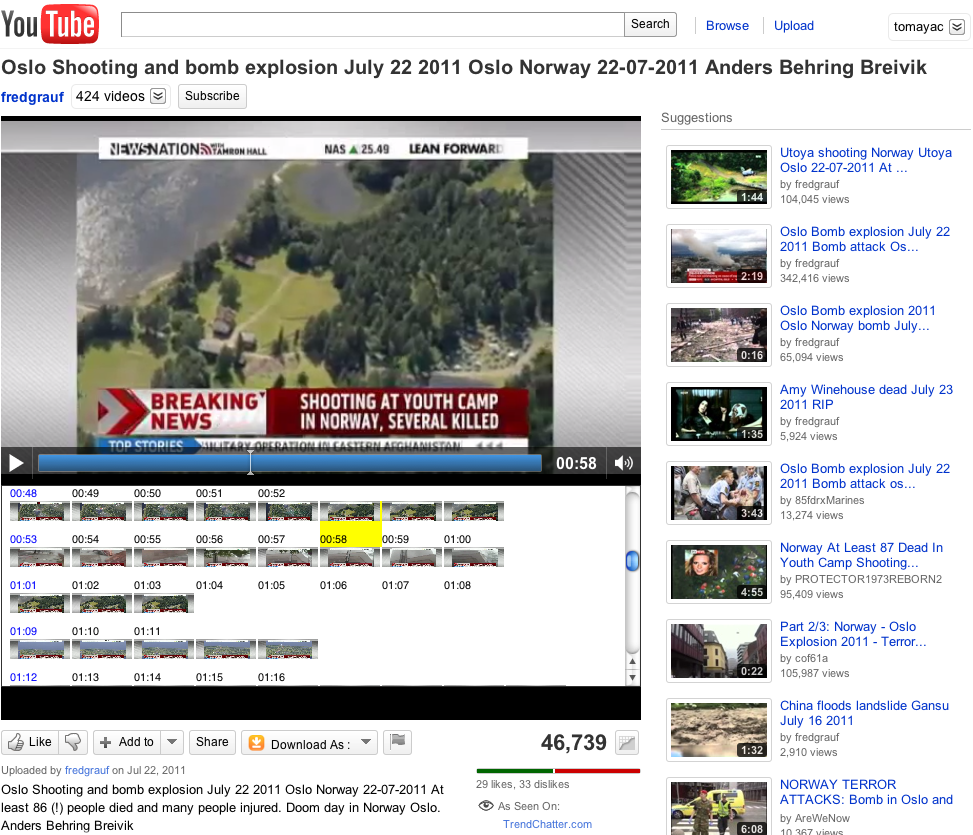
\includegraphics[width=0.8\linewidth]{./resources/screenshot.png}
\end{center}
   \caption{Screenshot of the YouTube scene detection browser extension.}
\label{fig:screenshot}
\end{figure*}

\section{Related Work} \label{sec:related-work}
We consider related work in the strictly related field of shot boundary detection and in the loosely related field of semantic enrichment of user-generated metadata on YouTube.

\subsection{Shot boundary detection}
Video fragments consist of shots, which are sequences of consecutive frames from a single viewpoint, representing an continuous action in time and space. The topic of shot boundary detection has already been described extensively in literature. While some specific issues still remain (notably gradual transitions and false positives due to large movement or illumination changes), the problem is considered resolved for many cases~\cite{Hanjalic2002, Yuan2007}. Below, we present an overview of several well-known categories of techniques.

Pixel comparison methods~\cite{Hampapur1994, Zhang1993} construct a discontinuity metric based on differences in color or intensity values of corresponding pixels in successive frames. This dependency on spatial location makes this technique very sensitive to (even global) motion. Various improvements have been suggested, such as prefiltering frames~\cite{Zhang1995}, but pixel-by-pixel comparison methods proved inferior in the end and have steered research to other directions.

A related method is histogram analysis~\cite{Smeaton1999}, where changes in frame histograms are used to justify the boundaries of shots. Their insensitivity to spatial information within a frame makes histograms less prone to partial and global movements in a scene. We can argue as a drawback that even visually very dissimilar frames can have similar overall histograms. For example, different shots in the same scene can be difficult to distinguish because of similar color information.

As a compromise, a third group of methods consisted of a trade-off between the above two techniques~\cite{Ahmed1999}. Different histograms of several, non-overlapping blocks are calculated for each frame, thereby categorizing different regions of the image with its own color-based, space-invariant fingerprint. The results are promising while computational complexity is kept to a minimum, which is why we have chosen a variation on this approach in this paper.

Other approaches to shot boundary detection include the comparison of mean and standard deviations of frame intensities~\cite{Lienhart1999}. Detection using other features such as edges~\cite{Zabih1995} and motion~\cite{Bouthemy1997} have also been proposed. However, Gargi \emph{et~al.}\ have shown that these more complex methods do not necessarily outperform histogram-based approaches~\cite{Gargi2000}. A detailed overview and comparison can be found in Yuan \emph{et~al.}~\cite{Yuan2007}. 

Another interesting track is shot boundary detection in the compressed domain~\cite{Yeo1995}, which is especially relevant for online video, as compression plays a major part herein. Unfortunately, even though this article focuses on online video, client-side manipulation of the raw, compressed stream would introduce a lot of computational overhead and make our implementation codec-dependent.

\subsection{Semantic Enrichment of User-Generated Metadata on YouTube}
In \cite{Choudhury:YouTube}, Choudhury et al. describe a framework for the semantic enrichment, ranking, and integration of Web video tags using Semantic Web technologies. In order to enrich the oftentimes sparse user-generated tag space, they use metadata like the recording time and location, or the video title and video description, but also social features such as playlists that a video appears in and related videos. Next, they rank the tags by their co-occurrence and in a final step interlink with DBpedia~\cite{Bizer:DBpedia}. While the semantic enrichment of YouTube metadata is of little help for the actual detection of scenes in a video, however, it still can help to visually ``iconify" them. For example, if it is known that a certain scene is about the DBpedia concept of the company Apple, Inc., this scene can then be visually represented by an icon in form of the Apple logo, in addition to the scene still frames.

In~\cite{semwebvid}, Steiner and Hausenblas describe a Web application that allows for the automatic generation of Resource Description Framework (RDF) video descriptions based on user-generated metadata such as title, description, tags, and closed captions. They enrich this textual information via multiple Natural Language Processing Web services in parallel in order to extract named entities. The detected named entities are interlinked with DBpedia concepts. While thanks to the closed captions their detected named entities are explicitly anchored to a point in the video, with our scene detection framework we can instead anchor named entities to scenes, which is context-wise oftentimes the better option.

Finally, Gao et al. propose in~\cite{Gao:2009} a theme-based thumbnail selection algorithm that explicitly models the visual characteristics of the underlying semantic video theme. This semantic model is constructed by finding the common features of relevant visual samples, which are obtained by querying a visual database with keywords associated with the video. Synergies between the approaches~\cite{Choudhury:YouTube,Gao:2009,semwebvid} and our current approach of scene detection with crowd-sourced hot spot detection are possible.

\section{Scene Detection Algorithm} \label{sec:details-of-algo}
In this Section, we discuss our scene detection algorithm.

\begin{figure}
\begin{center}
   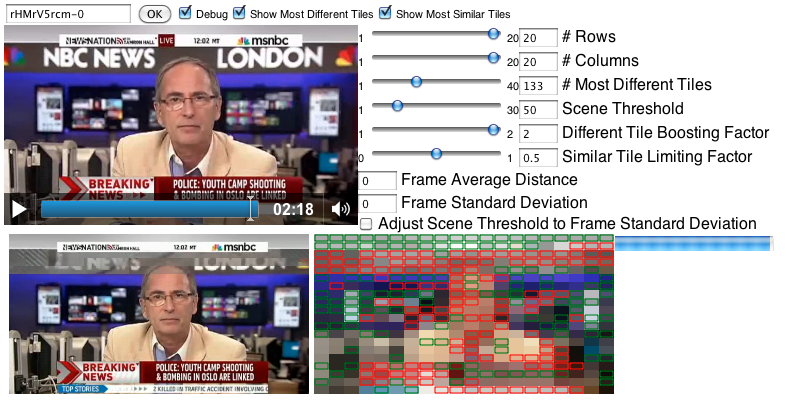
\includegraphics[width=1.0\linewidth]{./resources/algorithm.png}
\end{center}
   \caption{Debug view of the scene detection process. Red boxes highlight tiles with the most, green boxes with the least differences to the previous frame.}
\label{fig:algorithm}
\end{figure}

\section{Implementation Details} \label{sec:implementation}

\section{Evaluation} \label{sec:evaluation}

\section{Future Work and Conclusion} \label{sec:future-work-conclusion}

{\small
\bibliographystyle{ieee}
\bibliography{artemis2011}
}


\end{document}
